\documentclass{llncs}

% \usepackage{latexsym}
% \usepackage{amssymb}
\usepackage{graphicx}
\usepackage{cite}
\usepackage[normalem]{ulem}
\usepackage{xspace}
\usepackage{alltt}
\usepackage{amsmath}
\usepackage{extarrows}
\usepackage{url}
\usepackage[pdftex]{color}

% \usepackage{soul}
% \usepackage{multirow}
% \usepackage{listings}
% \setstcolor{red}
% \usepackage[utf8]{inputenc}
% \usepackage[T1]{fontenc}
% \usepackage{comment}
% \usepackage{times}

%%%%%%%%%%%%%%%%%%%%%%%%%%%%%%%%%%%%%%%%%%%%%%%%%%%%%%%%%%%%%%%%%%%%%%%

\newcommand{\hcinv}{\texttt{hc\_inversion}\xspace}
\newcommand{\coqdockw}[1]{\texttt{#1}}
\newcommand{\inversion}{\coqdockw{inversion}\xspace}
\newcommand{\inv}{\coqdockw{inv}\xspace}
\newcommand{\simlight}{\texttt{Simlight}\xspace}
\newcommand{\compcert}{\texttt{CompCert}\xspace}
\newcommand{\clight}{\texttt{Clight}\xspace}
\newcommand{\simsoc}{\texttt{SimSoC}\xspace}
\newcommand{\simsoccert}{\texttt{SimSoC-Cert}\xspace}
\newcommand{\stt}{\small\tt}
\newcommand{\why}{\texttt{Why}\xspace}
\newcommand{\whyML}{\texttt{WhyML}\xspace}
\newcommand{\whyCert}{\texttt{WhyCert}\xspace}
\newcommand{\framac}{\texttt{Frama-C}\xspace}

\newcommand{\SC}{SystemC\xspace}
\newcommand{\TLM}{TLM\xspace}

\newcommand{\insertfig}[1]{\input #1.pdftex_t}

\makeatletter
\renewcommand\subsubsection{\@startsection{subsubsection}{3}{\z@}%
                       {-18\p@ \@plus -4\p@ \@minus -4\p@}%
                       {0.5em \@plus 0.22em}%
                       {\normalfont\normalsize\bfseries\boldmath}}
\makeatother

%\setlength{\intextsep}{10pt plus 2pt minus 2pt}

\begin{document}
\setcounter{secnumdepth}{3}

%date not printed
\date{}

\title{SimSoC: A Fast, Proven Faithful, Full System Virtual Prototyping Framework}
\author{Vania Joloboff\inst{1} \and Jean\--Francois Monin\inst{2}
   \and Xiaomu Shi\inst{3}}
\institute{East China Normal University, Shanghai, China, INRIA, France\\
\email{vania.joloboff@inria.fr},\\
\and Grenoble University, France,\\
\email{jean-francois.monin@imag.fr},\\
\and Tsinghua University, China,\\
\email{xmshi@tsinghua.edu.cn}
}
\maketitle
\thispagestyle{empty}

\begin{abstract}

  This chapter presents the SimSoC virtual prototyping framework, a
  full system simulation framework, based on SystemC and Transaction
  Level Modeling. SimSoC takes as input a binary executable file,
  which can be a full operating system, and simulates the behavior of
  the target hardware on the host system. It is using internally
  dynamic binary translation from target code to host code to simulate
  the application software. A potential issue with simulators is that
  they might not accurately simulate the real hardware. We aimed at
  filling this gap by proving that the ARM instruction set simulator
  coded in C is a high fidelity implementation of the ARM
  architecture, using the Coq theorem prover, and starting from a
  formal architectural model in Coq. The first part of the chapter
  presents the general architecture and features of SimSoC.  The
  second part describes the proof of the ARM simulator.
\end{abstract}

\section{Introduction}

Computer modeling technologies have become powerful enough that one
can build a {\em virtual prototype} of the system under design.
Virtual prototypes make it possible to avoid the tedious and time
consuming process of making real hardware prototypes on which the
software has to be tested. They make it possible to develop an
emulated system that captures most, if not all, of the required
properties of the final system. A virtual prototype of a system
under design can be run and tested like the real one, the engineers
can exercise and verify the device properties.

In many engineering projects, some components are re-used from former
projects, assembled with modified ones, or new ones. It is necessary
to support emulation of new hardware components with enough detail,
integrated with existing simulation models, possibly coming from third
parties.  These requirements call for an integrated, modular, full
simulation environment where already proven components can be
simulated quickly, whereas new components under design can be tested
more thoroughly.  Modularity and fast prototyping also are important
aspects, to investigate alternative designs with easier re-use and
integration of third party IP’s.

The \simsoc project is developing a framework geared towards full
system virtual prototyping, able to simulate complete System-on-Chips
or boards. To this end, SimSoC provides a library of simulation models
for peripherals, interconnects, together with Instruction Set
Simulators (ISS) for the most common embeded systems processors. Each
ISS is designed as a SystemC module that issues transactions towards
the other models.

This chapter presents the overall system architecture and the \simsoc
ISS. To achieve fast processor simulation, the ISS technology uses
dynamic binary translation. The hardware models are standard SystemC
TLM abstractions and the simulator uses the standard SystemC
kernel. Therefore, the simulation host can be any commercial
off-the-shelf computer and yet provide reasonable simulation
performance.

A platform simulator such as \simsoc can be used to test critical
software such as cryptography or safety related embedded software. In
these situations, it is necessary to work with the full system
implementation, not only with the model specification. It is also
important to use a very faithful simulator in order to ensure that no
bias is introduced.  To achieve that goal, work was undertaken to
demonstrate how it can be verified that the simulated execution of a
binary program on the Instruction Set Simulator of a target
architecture indeed produces the expected results. This actually
requires several steps, to prove first that the translation from C
code to machine code is correct, and second that the simulation of the
machine code is also correct, that is, they all preserve the semantics
of the source code; together with the fact that all of these proofs
are verified using a theorem prover or proof checker, not subject to
human error in the proof elaboration or verification. The end result
is a faithful simulator.

The first part of this chapter describes the generic architecture of
the \simsoc framework with discussion of speed and accuracy. It
illustrates the different simulation modes supported by \simsoc, in
particular the standard interpretive mode and the two binary dynamic
translations modes. It also discusses performance estimation obtained
from simulation.

The second part of the chapter describes how a faithful, verified
simulator has been developed and proved. The technique presented here
partly relies on already existing tools, in particular the Coq proof
assistant, the Compcert C compiler, a certified compiler for the C
language, combined with our own work to prove the correctness of an
ARM Instruction Set Simulator, integrated within SimSoC.

\section{The SimSoC framework}

In order to simulate a complete hardware platform, one must simulate
simultaneously each of the individual components, and possibly advance
the clock that represents the simulated execution time. SystemC has
become the standard to represent and simulate hardware models, as it
is suitable for several levels of abstraction, from functional models
to synthetizable descriptions. It is defined by an IEEE
standard~\cite{systemc-lrm}, and comes with an open-source
implementation.  Transactional level modeling (TLM) refers both to a
level of abstraction~\cite{tlm-book} and to the SystemC-based library
used to implement transactional models~\cite{tlm-osci}. The
\emph{transaction} mechanism allows a process of an {\em initiator}
module to call methods exported by a {\em target} module, thus
allowing communication between TLM modules with very little
synchronization code.

SimSoC is implemented as a set of SystemC TLM modules and runs on top
of the SystemC kernel~\cite{apccas-2008}. The global architecture is
depicted in Figure~\ref{fig:simsoc-arch}. The hardware components are
modeled as TLM models, therefore the SimSoC simulation is driven by
the SystemC kernel.  The interconnection between components is an
abstract bus.  Each component simulated in the platform is abstracted
as a particular SystemC module. Each processor in the target platform
is implemented as an ISS that executes its instructions, which may
issue transactions towards other components, while maintaining the
processor state. A SimSoC ISS simulates the behavior of the processor
with instruction accuracy, not cycle accuracy. It emulates the
execution of instructions, exceptions, interrupts and the virtual to
physical memory mapping.
\begin{figure}[tbhp]
\centering
\scalebox{.5}{\insertfig{fig/simsoc_archi} }
\caption{SimSoC architecture}
\label{fig:simsoc-arch}
\end{figure}

The main task of an ISS is to carry out the computations that
correspond to each instruction of the simulated program. There are
several alternatives to achieve such simulation. In {\em interpretive
  simulation}, each instruction of the target program is fetched from
memory, decoded, and executed. This technique has been used in popular
ISS's such as Simplescalar~\cite{simplescalar-1997}. It is flexible
and easy to implement, but the simulation speed is slow as it wastes a
lot of time in decoding. A faster technique to implement an ISS is
{\em dynamic binary cached translation}.
\begin{figure}[th]
  \centering
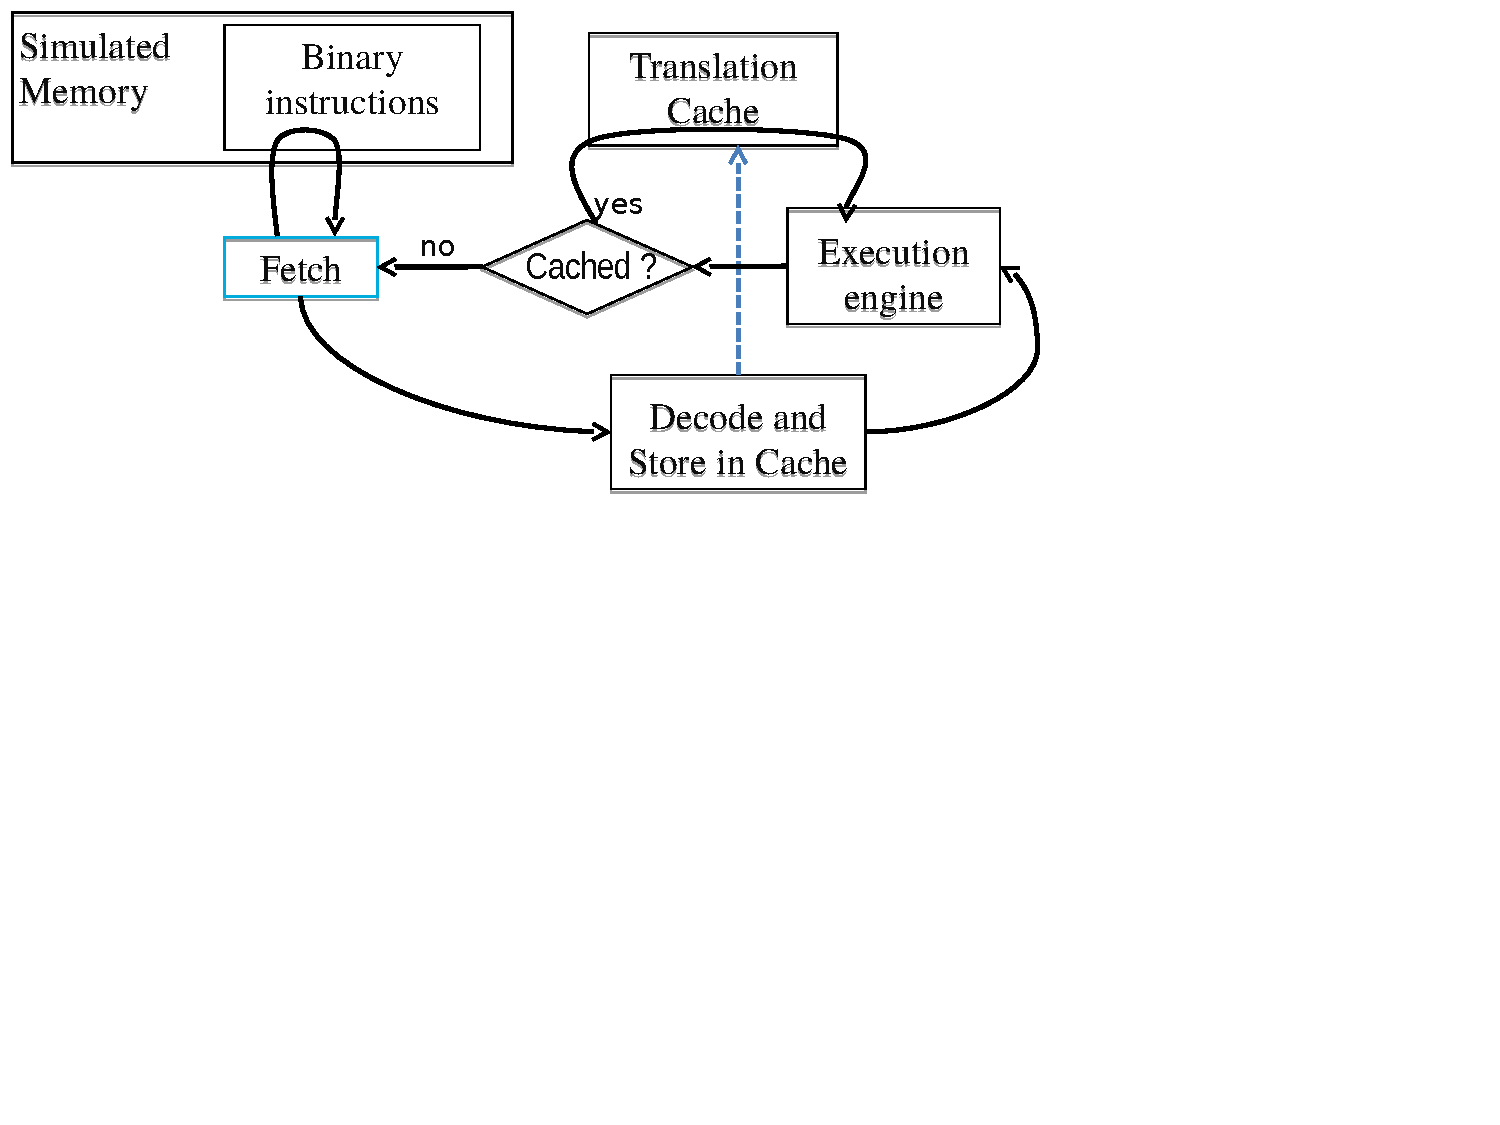
\includegraphics[scale=0.5, trim= 0mm 105mm 25mm 2mm, clip=true]
{fig/dyntrans.pdf}
  \caption{Dynamic Binary Translation}
  \label{fig:iss}
\end{figure}
With dynamic binary cached translation, illustrated in
Figure~\ref{fig:iss}, the target instructions are fetched from memory
at run-time but they are decoded only on the first execution and the
simulator translates these instructions into another representation,
which is stored into a cache. On further execution of the same
instructions, the translated cached version is used. If the code is
modified during run-time, the simulator must invalidate the cached
representation.  Although dynamic translation introduces a compile
time phase as part of an overall simulation session, this translation
latency is amortized over time and it has been commonly used
\cite{shade-cmelik-keppel,embra-witchell-rosenblum,reshadi-mishra-dynamicISS,scott-kumar-retargetable,vala-duesterwald-dynamo}.
Dynamic cached translators all work on the same model, however
translation simulators can be subdivided into three categories
according to the nature of the translated data and its usage, which we
will call here \textit{object oriented}, \textit{code generators}, or
\textit{micro-instructions based}.

In a \textit{micro-instructions} based ISS, each instruction is
translated into a sequence of pre-defined micro-instructions that are
stored into the cache. These pre-defined micro-instructions can be
considered as a very low level virtual machine that is run inside the
ISS, but this virtual machine is strongly related to the way the
simulated processor state is represented inside the ISS. In order to
translate each instruction, the parameters from each micro-instruction
must be extracted from the instruction (e.g. a constant for an
immediate load), and then the micro-instructions must be glued
together into a sequence. Because a whole sequence of target
instructions can be translated in a block of micro-instructions, the
execution is faster and higher simulation speed can be reached. Micro
instructions can be compiled in advance with highly optimizing
compilers \cite{qemu}. However, the micro-instructions must be linked
together and this process may be dependent upon target binary format
and host operating system, hence reducing portability of the ISS.

In the \textit{code generation} technique, the ISS translates the
target binary code into native host code.  As developing a complete
compiler technology is not realistic, the translators tend to leverage
off existing compiler technology.  either (i) by re-generating C code
that can be dynamically recompiled for the host machine
\cite{qin-zhu}, or (ii) by generating some intermediate language code
for which an existing back end compiler is used to generate the host
code \cite{dynamic-IL}, for example generate intermediate
representation of the popular GCC compiler and then use GCC back-end
to generate the code. The native code generation technique provides
higher performance when executing the simulated code. Edinburgh
University ISS claims to reach performance in the range of over
400~Mips \cite{jones-topham}. However, this performance must be
balanced with the throughput. Because dynamic translation is more
complex, it takes more time and the simulation time must be long
enough to amortize the translation time. This technology is worthwhile
when the virtual prototype tests are long enough, and sub-optimal when
running very short tests.

In an \textit{object oriented} ISS, the original instructions are
translated into a data structure of objects associated with function
calls. Each instruction can be translated into one object, each object
captures the variable data from the instruction and is bound to a
\textit{semantic function} that is called upon execution. With some
optimizations a sequence of instructions can possibly be translated
into one single object, for example a basic block. The advantage of an
object oriented ISS is that it is not so difficult to construct. In
fact using some appropriate input formalism the code of the object
classes and methods can often be generated. Using this technique, the
ISS is independent of the host operating system and independent of the
host processor, therefore easily portable. Because the semantic
functions are compiled in advance, a compiler with maximum
optimizations can be used and object oriented ISS'es can reach speed
above 100 Mips on a standard PC computer running at
about 3GHz.

The second mode of \simsoc is such an object oriented ISS. In this
dynamic translation mode, the decoder dynamically constructs an
intermediate representation that maps the binary instructions to a
data structure representing the program. The decoding phase mostly
amounts to allocating and initializing variables, and locating the
appropriate code from the pre-compiled library. In addition, the
translator can construct the control flow graph of the decoded
software into linked basic blocks, and achieve further optimization at
block level.

This mode explores two optimization techniques. First, it offloads the
compiling work by pre-compiling most of the simulation code with
maximum optimization. Second, it exploits \textit{partial evaluation},
a compiling optimization technique, also known as
\textit{specialization}~\cite{futamura}. The basic concept of
specialization is to transform a generic program $P$, when operating
on some data $d$ into a faster specialized program $Pd$ that executes
specifically for this data. Specialization can be advantageously used
in processor simulation, because data can often be computed at
decoding time, and a specialized version of the generic instruction
can be used to execute it. The simulation code then uses fewer tests,
fewer memory accesses and more immediate instructions. This technique
has been used to some extent in the IC-CS simulator
\cite{naul-braun-jit-iccs}.

Conceptually, specializing completely the instruction set would mean
that for every possible parameter of an instruction (each bit field),
there would be a specialized function computing the result.
Potentially there are at most $2^{32}$ specializations of a 32-bit
instruction set, which would lead to a huge amount of specialized
code.  In practice however, there are reserved encoding bits, many
binary configurations are illegal, and overall some instructions are
more frequently executed than others. By specializing only the most
significant parameters and the most frequently used instructions to a
higher degree than the less frequent ones, one can reduce the number
of specialized functions to a manageable amount of code.

Let us consider the example drawn from the ARM architecture ISS, the
{\tt ADD} instruction, noted in assembly language as: {\tt
  ADD\{<cond>\}\{S\} <Rd> ,<Rn>, <operand>}. Its semantic is described
in ARM Architecture Reference Manual~\cite{arm-ref-book} shown in
Figure \ref{fig:add-pseudocode}.
\begin{figure}[h]
  \centering
\begin{verbatim}
if ConditionPassed (cond) then
 Rd = Rn + operand
  if S == 1 and Rd == R15 then
    CPSR = SPSR
  else if S == 1 then
    N Flag = Rd[31]
    Z Flag = if Rd == 0 then 1 else 0
    C Flag = CarryFrom(Rn + operand)
    V Flag = OverflowFrom(Rn + operand)
\end{verbatim}
  \caption{ARM ADD instruction}
  \label{fig:add-pseudocode}
\end{figure}

The {\tt S} bit indicates whether the instruction updates the Current
Process Status Register (CPSR) or not. There are 11 addressing modes
used to calculate the operand in an ARM data-processing instruction,
such as immediate, using a register, shifted or non shifted, and so
on. The operand mode and the addressing mode are specified in the
instruction, they are discovered at decoding time. In order to
maximize performance, one can use many specialized semantic functions
that each carry the very specific task discovered, instead of
executing the slower generic one. In order to test multiple
specialization possibilities, \simsoc includes a generator that can
generate the specialized functions automatically based on input
specifications. For example, it can specialize the functions on the
condition code, the {\tt S} bit, the operand mode and the registers of
data-processing instructions. As an example, the generated semantic
function below is the {\tt ADD} instruction simulation code when the
condition code is {\tt EQ}, the {\tt S} bit is 0, and the operand is
not shifted.
\begin{verbatim}
PseudoStatus add_Ceq_S0_Mreg
(Processor &proc, PseudoInstruction &pi)
{ if (!proc.cpsr.z) return OK;
  uint32_t tmp = proc.regs[pi.dpi.Rn];
  uint32_t opv = proc.regs[pi.dpi.Rm];
  uint32_t r = tmp + opv;
  proc.regs[pi.dpi.Rd] = r;
  return OK; }
\end{verbatim}

In interpretive mode, one function is used to implement the ADD
operation.  In contrast, in the specialized mode, 330 specialized
functions are used to implement ADD corresponding to: 15 (condition
code) * 2 ({\tt S} bit) * 11 (operand mode).  For the experiment
below~\cite{simsoc-csee2008}, specialization is used to a limited
extent, with no specialization on the registers and no specialization
on the condition codes. Table \ref{tab:dynamic-translation} shows the
speed improvement on typical benchmarks between the interpreted mode
(D0), a simple dynamic translation cache (D1) and the version using
partial interpretation (D2).

\begin{table}[tbhp]
%% \vspace*{-2ex}
\caption{Comparison of interpretive and dynamic translation}
\label{tab:dynamic-translation}
\centering
\begin{tabular}{|c|c|c|c|}\cline{2-4}
\multicolumn{1}{c|}{}        & D0 & D1 & D2 \\ \hline
crypto.a0.x  & 522 s & 221 s & 57.6 s \\
arm32, no opt. & 6.62 Mips & 15.6 Mips &  59.9 Mips \\ \hline
crypto.a3.x  & 139 s & 62.2 s & 11.6 s \\
arm32, with opt. & 6.84 Mips & 15.3 Mips & 82.3 Mips \\ \hline
crypto.t0.x & 1996 s & 576 s & 153 s \\
thumb, no opt. & 5.01 Mips & 17.3 Mips & 65.4 Mips \\ \hline
crypto.t3.x & 299 s & 90.6 s & 26.6 s \\
thumb, with opt. & 5.40 Mips & 17.8 Mips & 60.7 Mips \\ \hline
loop.a0.x   & 18.2 s & 9.26 s & 1.57 s \\
arm32, no opt. & 7.37 Mips & 14.5 Mips & 85.4 Mips\\ \hline
loop.t0.x  & 38.1 s & 12.1 s & 2.49 s \\
thumb, no opt. & 4.84 Mips & 15.2 Mips & 74.1 Mips \\ \hline
\end{tabular}
\end{table}

To ever increase simulation speed, a third code generation translation
mode was added to \simsoc, which uses the LLVM~\cite{llvm-2004}
library. LLVM is a Low Level Virtual Machine that has been designed to
serve as intermediate representation in compilers suitable for complex
optimizations. It consists in an abstract instruction set, each
instruction having well defined semantics. An LLVM program can be
interpreted directly using the LLVM interpreter, or compiled to
machine code. The code generation can be done either with a JIT
compiler or a batch compiling phase. LLVM contains a complete set of
high-level compiler optimizations, ranging from simple scalar
simplifications to complex loop transformations.

The LLVM dynamic translator in \simsoc translates on the fly target
basic blocks into LLVM functions, yet again using a precompiled
library in LLVM bitcode. Then one can use the existing LLVM optimizer
and Just-In-Time compiler to generate native code, as shown in
Figure~\ref{fig:dyntrans-native}.  The translation time from target
code to LLVM, next from LLVM to native, can become lengthy and
ultimately defeat the speed-up in execution time. Thus, the ISS
actually mixes translation modes with a method to evaluate and select
only ``hot path'' code so that the LLVM translation is not systematic,
but only operates on such hot paths, the remaining code being
simulated with the standard translation. This effectively provides
overall faster simulation~\cite{simsoc-llvm-2011}.
\begin{figure}[!ht]
% [tbhp]
  \centering
  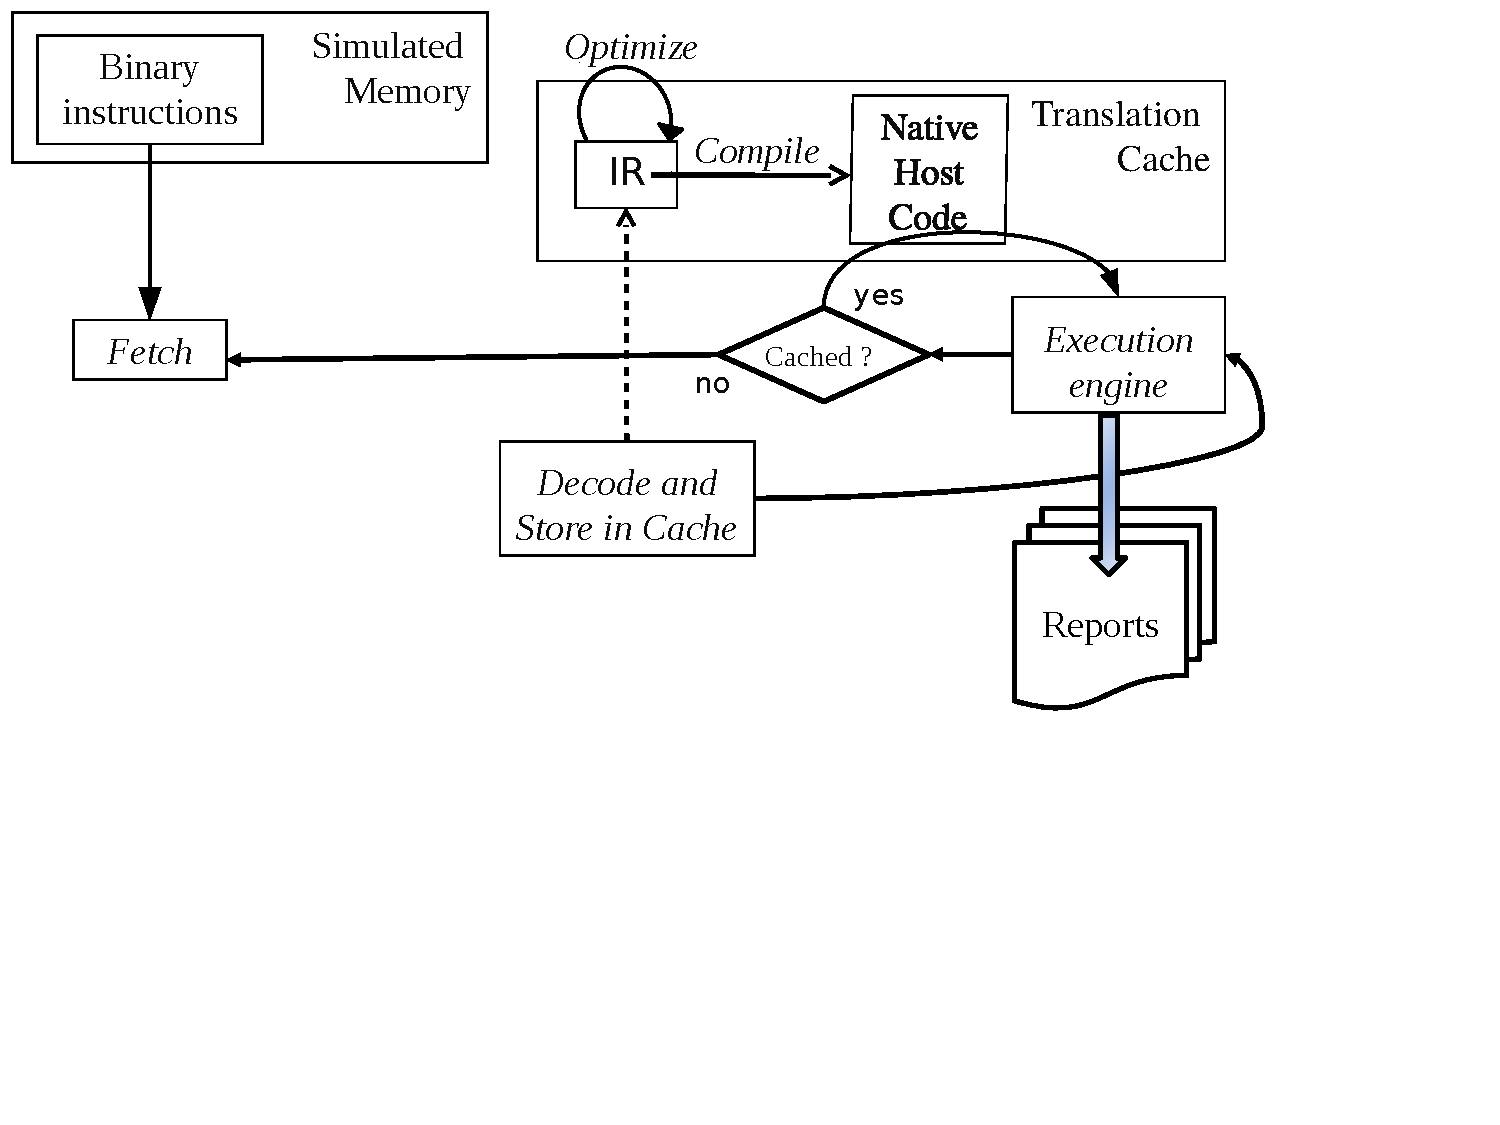
\includegraphics[scale=0.5, trim = 10mm 75mm 40mm 2mm clip=true]{fig/dyntrans-native.pdf}
  \caption{Dynamic binary translation to native code with LLVM}
  \label{fig:dyntrans-native}
\end{figure}

In the native code translation mode, the translation-unit is a
\textit{Basic block}, a straight sequence of code with only one entry
point and only one exit, a branch instruction at the end. By
construction, all instructions from a basic block will certainly be
executed when it is entered. Each basic block can be compiled into a
linear simulation function, which allows fast translation and
simulation.  Below is an example of a basic block of PowerPC
instructions to be translated into an LLVM function:
%{\small
\begin{alltt}
  \textbf{addis} r9, r0, 385
  \textbf{lwz  } r0, 1076 (r9)
  \textbf{or   } r1, r0, r0
  \textbf{bl   } 0xffffff70
\end{alltt}
%}

To translate a basic block to LLVM, the translator creates an LLVM
function, containing a single LLVM block {\tt entry}. This LLVM
function has a parameter {\tt \%proc} that holds the processor
state. Then, for each instruction, it generates a call to the
corresponding execution function, which must be defined by existing
LLVM code. The implementations of these LLVM functions are stored in a
LLVM bitcode library, whose generation is explained below.  For
example, the instructions {\tt addis} and {\tt lwz} are translated to
specialized llvm function calls to corresponding functions {\tt
  \@addis\_ra0} and {\tt \@lwz\_raS}. Each instruction is followed by
a function call to update the value of the PC register. The status
returned by an execution function tells whether a branch has occurred;
by definition, all status but the last tell that no branch occurred.
Thus, the basic block above is translated to the following LLVM
function.
%{\small
\begin{alltt}
  \textbf{define} void @\textbf{bb_687} (\%"struct.Proc"* \%proc) \verb|{|
  \textbf{entry}:
   \%status = call i32 @\textbf{addis\_ra0}(\%"struct.
                   Proc"* \%proc, i8 9, i32 385)
   call void @\textbf{inc_pc}(\%"struct.Proc"* \%proc)
   \%status1 = call i32 @\textbf{lwz_raS}(\%"struct.
            Proc"* %proc, i8 0, i8 9, i32 1076)
   call void @\textbf{inc_pc}(\%"struct.Proc"* \%proc)
   \%status2 = call i32 @\textbf{or}(\%"struct.
                Proc"* \%proc, i8 0, i8 1, i8 0)
   call void @\textbf{inc_pc}(\%"struct.Proc"* \%proc)
   \%\textbf{status3} = call i32 @\textbf{bl}(\%"struct.
                        Proc"* \%proc, i32 -144)
   call void @\textbf{inc_pc_if_no_branch}(i32 \%\textbf{status3},
                         \%"struct.Proc"* \%proc)
   ret void
 \verb|}|
\end{alltt}
%}

When a basic block has been constructed, one can use LLVM optimization
functions at will. In particular, the {\em AlwaysInline} optimization
is systematically called first so that all the code of the execution
functions is actually inlined, and thus available for further
optimizations.  Next, other optimizations can be accomplished. For
example, LLVM will reduce the $K$ successive calls to {\tt inc\_pc()}
inlined functions into a single addition of $K\times 4$ to the PC when
the PC variable is never read.  In general, after the {\em
  AlwaysInline} pass, the LLVM optimization passes named {\em
  GVNPass}, {\em InstructionCombiningPass}, {\em
  CFGSimplificationPass}, and {\em DeadStoreEliminationPass} are also
applied.

After the LLVM optimization passes, the LLVM JIT compiler is used to
compile LLVM bitcode into host binary code. Then the instruction cache
is updated so that the native code is called instead of the simulation
function.  As it is much easier to write C++ code than LLVM bitcode,
to obtain the LLVM library, a library of C++ functions is compiled
into a LLVM bitcode library prior to simulation. As an example, here
is the C++ code implementing the PowerPC {\em add} instruction:

{\small
\begin{alltt}
  extern "C" PseudoStatus \textbf{ppc_add}
            (Proc &proc, u8 rt, u8 ra, u8 rb) \verb|{|
   const uint32_t a = proc.cpu.gpr[ra];
   const uint32_t b = proc.cpu.gpr[rb];
   proc.cpu.gpr[rt] = a+b;
   return OK;
 \verb|}|
\end{alltt}
}

\noindent And here is the LLVM bitcode generated by {\tt llvm-g++}:

{\small
\begin{alltt}
  \textbf{define} i32 @\textbf{ppc_add}(\%"struct.Proc"* nocapture
         \%proc, i8 zeroext \%rt, i8 zeroext \%ra,
                     i8 zeroext \%rb) nounwind \verb|{|
  entry:
   \%0 = zext i8 \%ra to i64;
   \%1 = geteleptr inbounds \%"struct.Proc"*
            \%proc, i64 0, i32 2, i32 4, i64 \%0;
   \%2 = \textbf{load} i32* \%1, align 4;
   \%3 = zext i8 \%rb to i64;
   \%4 = geteleptr inbounds \%"struct.Proc"*
            \%proc, i64 0, i32 2, i32 4, i64 \%3;
   \%5 = \textbf{load} i32* \%4, align 4;
   \%6 = \textbf{add} i32 \%5, \%2;
   \%7 = zext i8 \%rt to i64;
   \%8 = geteleptr inbounds \%"struct.Proc"*
            \%proc, i64 0, i32 2, i32 4, i64 \%7;
   \textbf{store} i32 \%6, i32* \%8, align 4
   ret i32 0
 \verb|}|
\end{alltt}}

Another translation mode with larger translation units has also been
experimented, by dynamically determining strongly coupled basic
blocks in the control flow graph. Finally, in order to benefit from
multi-core simulation hosts, a distributed dynamic translation
mechanism has been experimented.  In that configuration, the native
code translation is achieved by a separate dynamic translation server,
that runs concurrently with the ISS on other processors. This work has
been described in \cite{amasbt-2012}.

\subsection{Performance Estimate}

SimSoC version released in open source is Loosely Timed. It advances
the clock using the quantum method. Each instruction is assumed to
execute in some time, which defaults to a constant time. Each quantum
of N instructions (a parameter) the clock is advanced by the amount of
execution time for that quantum. This method makes it possible to run
application software with timers and have some idea of the software
performance, but it cannot be used for worse case analysis or fine
grain performance estimates. However many applications want to have
performance estimates.

As cycle accurate simulators are much too slow to
be usable in an iterative, agile, development cycle, people have
seeked other solution to obtain performance estimates.
Attention has turned towards {\em sampling}, in which
a few chunks of code sequences are selected and
analyzed.  Then statistical methods are used to generate performance
estimates.  Popular representatives of sampling methods are
Simpoint\cite{simpoint-2004}, SMARTS\cite{smarts-2003} and
EXPERT\cite{expert-2004}. These systems differ mostly in the manner
the samples are selected, in size and frequency. Sampling techniques
can provide fairly accurate performance prediction with a high
probability but may also generate very large data files, and
face the issue of initializing state before running the sample.

The idea of "Approximately Timed" is to provide estimates while
running entirely the code, not using statistical methods, by
exercising abstract models of the architecture, but with a simulation
speed that is an order of magnitude faster than a cycle accurate one,
yet obtaining measurements that are less than a bounded margin error
from the real hardware performance.

Modern processors have complex architectures. They can execute
theoretically a certain number of instructions per clock cycle. There
are however several cases where the instruction flow is disrupted,
introducing delays in the computation. Well known causes of delays are
\begin{itemize}
\item There are cache misses. Either data cache miss, or the next
  instruction to be executed is not available.
\item
  The pipe line is stalled. Instructions are executed in a pipe line
  to achieve multiple operations in each pipe line issue on each
  clock cycle, but the pipe line may get stalled in some
  circumstances.
\item
  There are wait states because of communication with peripherals.
\end{itemize}

Approximately Timed simulation has been explored in the \simsoc
project, with the idea to simulate enough of the processes causing the
delays to estimate them, though not simulating the exact hardware
processes of the caches and pipe line and I/Os. The approach consists
in developing a higher abstraction model of the processor (than the CA
models) that still execute instructions using fast SystemC/TLM code,
but in parallel maintains some architecture state to measure the
delays introduced by cache misses and pipe line stalls. These models
do not mimic the architecture, they only measure the delays.  A case
study has been done with a model of the instruction cache and the data
cache and the pipe line, for a sample of a Power architecture
processor (e200). Our method consists in evaluating the delays with the
following approach:
\begin{itemize}
\item approximate the delays created by the instruction cache misses,
  and (pre)fetches. A cache simulator has been implemented  that does
  not simulate the specific hardware architecture cache in detail, but
  uses an algorithm that reproduces the cache behavior to tell whether
  there is a cache hit or miss. The instruction buffer is also
  simulated in an abstract way so that we can compute whether or not
  the pipe line is fed with instructions.
\item build a model of the pipe line architecture that makes it possible
to evaluate delays without reproducing in detail the hardware behavior.
\item evaluate with a high precision the most frequently executed
  code (the hot blocks), and use a lower precision for the code that
  is rarely used (the cold blocks).
\item perform a static analysis of basic blocks only once, assuming
  that future execution of these blocks will approximately take the
  same number of cycles (except for the cache misses).
\item rely on Transaction Level Modeling interface to obtain I/O delays
The delays related to bus arbitration and interconnect access can be
captured by TLM transactions as of the TLM~2 standard. A SimSoC ISS
relies upon TLM interface to the interconnect to provide timing
delays.
\end{itemize}

This Approximately Timed method purposedly makes errors at
least on the following points:
\begin{itemize}
\item instruction prefetch is not computed exactly at the same time as
  the prefetch in the real hardware. In this method the effect of
  pre-fetch is computed at block level. For example, it may be the
  case that at the time of a real prefetch, the interconnect is busy
  working for other components such as peripherals or coprocessors. In
  our simulation, the components will use the interconnect but may be
  at a different time (may be the same, by chance) therefore the delay
  returned by the interconnect interface is not the real delay that
  will occur.

\item the same is true for memory reads and writes. The cache
  simulation does not simulate exactly the hardware
  cache. It only knows when there is cache miss and then generates a
  transaction.  As the interconnect is not solicited at the same time
  in the simulation than in the real chip, there is a possible error.

\item Additional delays introduced by variable length instructions like
  multiply and divide are ignored. A constant average factor is used.
\item As mentioned above, the simulator does not maintain an accurate
  state of the micro-achitecture, there are loopholes in the
  transition between basic blocks.
\end{itemize}

This has resulted in good approximation while reducing the
simulation speed in acceptable manner for the Power e200 processor
model used in our case study. For the software developers who want to
quickly compare various software/hardware implementations, fixing all
of these error sources would take a very significant simulation
overhead, whereas the error introduced fits in the approximation
objectives.

%%%%%%%%%%%%%%%%%%%%%%%%%%%%%%%%%%%%%%%%%%%%%%%%%%%%%%%%%%%%%%%%%%%%%%%%%%%%%
\section{Faithful Simulation}
\label{verification}

\subsection{Objective}

In many applications nowadays, virtual prototyping is used to design,
develop and test new applications. Most of these virtual prototypes
include an Instruction Set Simulator (ISS) to simulate the target
processor. The ISS runs the target executable binary code in emulating
the hardware and generate the outputs that the executable should
produce when run on the target platform. An ISS can be used for
example to optimize algorithms such as cryptographic software, or to
debug new compiler developments, or in the design of many embedded
systems applications.  Instead of using real hardware prototypes,
simulated platforms are more convenient and less expensive.  Then, it
is is important to be sure that the simulator used is faithful to the
hardware that it emulates.  A {\em faithful ISS} must produce exactly
the same results as the executable would if run on hardware
implementation of the instruction set, and this guarantee must be
proven.

We have started a first attempt to formally verify that the execution
of a program on our Instruction Set Simulator for the target ARM
architecture indeed produces the expected results, to be certain that
the data output from the simulator, the final processor and memory
states are indeed identical to the result obtained with the real
hardware. This requires sequential steps, to prove first that the
translation from the C code of the simulator to the simulation machine
is correct, and second that the simulation of the target machine code
is also correct, that is, it preserves the semantics of the computer
architecture, together with the fact that all of these proofs are
verified using a theorem prover, or proof checker, not subject to
human error in the proof elaboration or verification.

The paragraphs below are organized as follows. The next paragraph
\ref{background} provides the formal verification background in our
context.  Paragraph \ref{tools} describes the tools that have been
used, in particular the Compcert~C compiler, a certified compiler for
the C language and the Coq proof assistant.  The proof structure
presented afterwards sketches our contribution to prove the
correctness of an ARM Instruction Set Simulator. In summary, the
method consists in proving each instruction of the instruction set
independently, by proving that the execution of the C code simulating
an instruction yields identical result to that obtained by a formal
executable model of the architecture.

Each independent proof requires using a number of lemmas from a
generic lemmas library and usage of a new inversion tactics in the
theorem prover.  Finally, our conclusion mentions lessons learned and
directions for future work.


%%%%%%%%%%%%%%%%%%%%%%%%%%%%%%%%%%%%%%%%%%%%%%%%%%%%%%%%%%%%%%%%%%%%%%%%%%%%%
\subsection{Formal Verification Background} %
\label{background}

Program certification has to be based on a formal model of the program
under study.  Such a formal model is itself derived from a formal
semantics of the programming language.
Axiomatic semantics and Hoare logic %\cite{Floyd67,Hoare-1969}
have been widely used for proving the correctness of programs.  For
imperative programming languages such as C, a possible approach is to
consider tools based on axiomatic semantics, like
\framac~\cite{canet2009value}, a framework for a set of interoperable
program analyzers for C. Most of the modules integrated inside rely on
ACSL (ANSI/ISO C Specification Language), a specification language
based on an axiomatic semantics for C.
% ACSL is powerful enough to
%express axiomatizations directly at the level of the C program.  State
%labels can be defined to denote a program control point, and can then
% be used in logic functions and predicates.

\framac software leverages off from \why technology
\cite{bobot2011why3,filliatre07cav}, a platform for deductive program
verification, which is an implementation of Dijkstra's calculus of
weakest preconditions.  \why compiles annotated C code into an
intermediate language.  The result is given as input to the VC
(Verification Conditions) generator, which produces formulas to be
sent to both automatic provers or interactive provers like Coq.

In our case of verifying an instruction set implementation, one has to
deal with a very large specification including complex features of the
C language. A framework is required that is rich enough to make the
specification manageable, using abstraction mechanisms for instance,
and in which an accurate definition of C features is available.  As we
need to verify specific properties referring to a formal version of
the ARM architecture, operational semantics offer a more concrete
approach to program semantics as it is based on states. The behavior
of a piece of program corresponds to a transition between abstract
states.  This transition relation makes it possible to define the
execution of programs by a mathematical computation \emph{relation}.
This approach is quite convenient for proving the correctness of
compilers, using operational semantics for the source and target
languages (and, possibly intermediate languages).

Operational semantics are used in \compcert (described below) to
define the execution of C programs, or more precisely programs in the
subset of C considered by the \compcert project.  The work presented
in this paper is based on this approach.  Interesting examples are
given by Brian Campbell in the CerCo
project~\cite{campbell2012executable}, in order to show that the
evaluation order constraints in C are lax and not uniform.

A very significant verification work has been done to prove the SEL4
operating system\cite{sel4-sosp2009}. It is comparable to our work in
that they have considered a C implementation.  The main difference is
that they have not considered operational semantics of C, but deduced
the proof obligations from the C code, considering the compiler and
the architecture as correct. In our work, we believe that the subset
of C accepted by \compcert is even larger than the subset accepted in
SEL4.

Regarding formalization and proofs related to an instruction set, a
Java byte code verifier has been proved by Cornelia
Pusch\cite{pusch-1999}, the Power architecture semantics has been
formally specified in \cite{alglave-2009}, and closer to our work, the
computer science laboratory in Cambridge University has used HOL4 to
formalize the instruction set architecture of ARM~\cite{FoxM10}. The
objective of their work was to verify an implementation of the ARM
architecture with \emph{logical gates}, whereas we consider a ARM
architecture simulator coded in C.  Reusing the work done at Cambridge
in \cite{FoxM10} was considered.  But, because our approach requires a
certified C compiler, in this case \compcert C, which is itself coded
in Coq, it would have required us to translate all of the C
operational semantics as well, which would have been error prone, not
to mention the very large effort. It was more convenient to develop
our formal model and our proofs in Coq.

%%%%%%%%%%%%%%%%%%%%%%%%%%%%%%%%%%%%%%%%%%%%%%%%%%%%%%%%%%%%%%%%%%%%%%%%%%%%%
\subsection{Background Tools} %
\label{tools}

The formal verification of the ISS is achieved by using two other
existing software tools that have been themselves verified, namely Coq
and CompCert~C.

\subsubsection{Coq}
Coq~\cite{coqart} is an interactive theorem prover, implemented in
OCaml. It allows the expression of mathematical assertions,
mechanically checks proofs of these assertions, helps to discover
formal proofs, and may extract a certified program from the
constructive proof of its formal specification.  Coq can also be
presented as a dependently typed $\lambda$-calculus (or functional
language).  For a detailed presentation, the reader can
consult~\cite{coqmanual} or~\cite{coqart}.  Coq proofs are typed
functions and checking the correctness of a proof boils down to
type-checking.
% For example, a proof term of type $\forall~n: nat,~P\,
% n~\rightarrow Q\, n$ is a function $fun~(n:nat) (p:P\:n)$ which takes
% a natural number $n$ and a proof $p$ of $P\:n$ as arguments and
% returns a proof of $Q\:n$.

The logic supported by Coq includes arithmetic, therefore it is too
rich to be decidable.
% However, type-checking, in particular, checking
% the correctness of a proof, is decidable.
As full automation is not
possible for generating proofs, human interaction is essential.  The
latter is realized by \emph{proof scripts}, which are sequences of
commands for building a proof step by step.  Coq also provides
built-in {\em tactics} implementing various decision procedures for
suitable fragments of the calculus of inductive constructions and a
language % called \texttt{Ltac} % unused in this paper
which can be used for automating the search of proofs and shortening
scripts.

When a proof has been interactively developed, Coq automatically
verifies the proof, or possibly signals where errors are located.
Our work has consisted in developing proofs demonstrating that
the C functions simulating the behavior of the ARM processor
indeed implement the ARM architecture semantics.

\subsubsection{Compert-C}
\compcert is a formally verified compiler for the C programming
language provided by INRIA~\cite{ccc,Leroy-Compcert-CACM}, which
currently targets Power, ARM and 32-bit x86 architectures.  The
compiler is specified, programmed, and proved in Coq. It aims to be
used for programming embedded systems requiring high reliability.
% and is always better than that of gcc without optimizations.
%
% It has a complex translation chain of eleven steps, from C source code
% into assembly code. Every internal representation has its own syntax
% and semantics defined in Coq.
% It is formally verified in the sense that
The generated assembly code is proved to behave exactly the
same as the input C program, according to a formally defined
operational semantics of the language.

A key point is that we are considering here C programs compliant with
the definition of ISO-C 99 standard of {\em correct C programs}.
Indeed the ISO-C standard identifies many constructions that are
syntactically correct, but have undefined semantics such as
\texttt{a[i++] = i;}. The document identifies about one hundred
such constructions, and says that a C compiler in that case basically
may choose its own interpretation of the abstract syntax,
resulting in \textit{unspecified behavior}.
This is very important in our work. All of the C code implementing the
ISS is correct with respect to the ISO C standard, meaning that it does
not contain any construction with unspecified behavior. Compcert-C
does not accept such ill-defined expressions and only well formed
programs can be translated according to the formal, unambiguous,
semantics. All of the C code considered here has unique and
well defined semantics. We need to prove that it implements the ARM
semantics, but we do not need to worry about multiple interpretations.

Three parts of \compcert C are used in this work. The first is that we
use the correct machine code generated by the C compiler.  The second
is the C language operational semantics in Coq
% (its syntax and semantics),
from which we get a formal model of the program.
Third, we use the \compcert Coq library for words,
half-words, bytes etc., and bitwise operations
% and lemmas to describe their properties.
% In our Coq model, we also use these low level
% representations and operations
to describe the instruction set model. These low level functions have
been proven already in \compcert, so we can safely re-use them.

It must be noted that the C code of an ISS does not use functions from
the C library that invoke the operating system, such as
\texttt{gettimeofday()},
% and the
% simulated memory is represented by host memory that is allocated
%upfront when the simulator starts.
It uses a very limited number of
functions from the C library such as \texttt{memset()} or
\texttt{memcpy()}.  \compcert provides the formalized properties of
such built-in external functions, so we can reason formally on their
potential side effects in our proofs.


%%%%%%%%%%%%%%%%%%%%%%%%%%%%%%%%%%%%%%%%%%%%%%%%%%%%%%%%%%%%%%%%%%%%%%%%%%%%%
\subsection{Verified Simulation}
\label{method}
The general objective is to obtain a verified simulator is illustrated in
Figure~\ref{fig:diagram}.  Considering the ARM architecture, we need
to have the following:\begin{itemize}\itemsep=0pt
\item a formal model of the ARM instruction set.
\item an instruction set simulator of the ARM arcchitecture coded in
  the (\compcert) C programming language.
\item a formal operational semantics of the ISS. As shown in
  Figure~\ref{fig:diagram}, from the ISS source code in C, we can
  obtain through \compcert C on one hand
  the Coq formal semantics of the compiled C program constructed by
  \compcert, since the intermediate representation of the C compiler
  is a Coq representation
%  or alternatively
  and, on the other hand,
  the verified machine code,
  which conforms to this operational semantics as guaranteed by CompCert.
  We use both, the compiled machine code to
  run simulations, and the formal semantics for the proof.
\item prove, using the Coq proof assistant, that the resulting ISS semantics
  indeed implement the formal model of the ARM processor, which boils
  down to verifying that the semantics of the simulator accurately
  modifies the processor (and memory) state representation at each
  step and ends up in results that comply with the
  formal model of the ARM architecture.
\end{itemize}
\begin{figure}
% TODO remettre trim left bottom right top
\hfil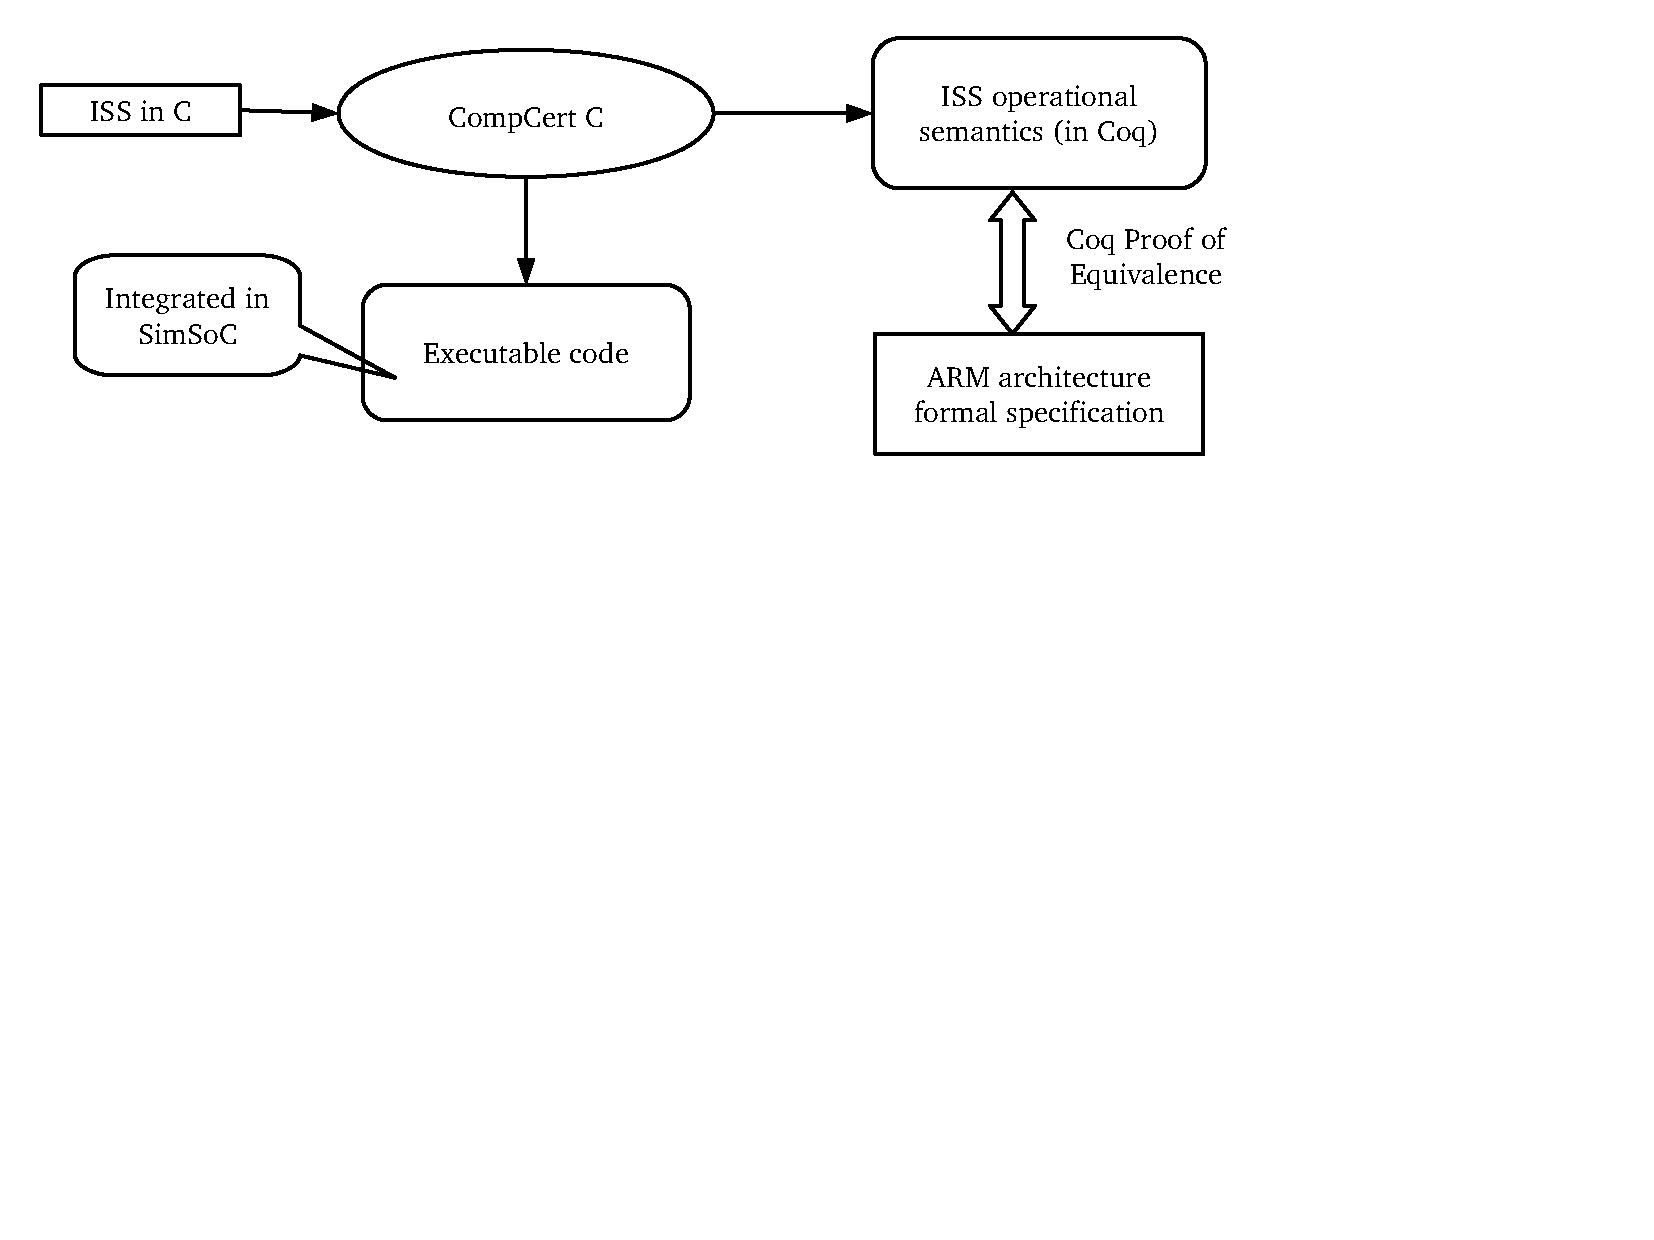
\includegraphics[width=0.9\linewidth, trim= 7mm 133mm 55mm 6mm, clip=true]
{fig/newdiag.pdf}
\caption{Overall goal}
\label{fig:diagram}
\end{figure}

These steps are described in the following paragraphs.


\subsubsection{Constructing the formal model}
Ideally the formal specification of the ARM architecture should be
provided by the vendor. But it is not the case,
an issue already raised
in the work with HOL4 mentioned above~\cite{FoxM10}.
% such a formal model is not available on their web site,
%% hence we had to build one
%% The only document available is
%% the ARM reference manual \cite{arm6refman}.
% (version 6 for this work).
We decided to derive
% So, it was elected to define
the formal
model of ARM architecture in Coq from the architecture
reference manual as output of a semi-automated process. The main
relevant chapters of the manual are:
\begin{itemize}
\item
\texttt{Programmer's Model} introduces the main features in ARMv6 architecture,
the data types, registers, exceptions, etc;
\item
\texttt{The ARM Instruction Set}
explains the instruction encoding in general and puts the instructions in
categories;
\item \texttt{ARM Instructions} lists all the ARM instructions in
  ARMv6 architecture in alphabetical order and the \texttt{ARM
    Addressing modes} section explains the five kinds of
  addressing modes.
\end{itemize}

There are 147 ARM instructions in the ARM V6 architecture.  For each
instruction, the manual provides its encoding table, its syntax, a
piece of pseudo-code explaining its own operation, its exceptions,
usage, and notes.
% %Need room...
%  Except the semi-formal pseudo-code, everything else
% is written in natural language.
%
Three kinds of information are extracted for each ARM operation: its
binary encoding format, the corresponding assembly syntax, and the
instruction semantics, which is an algorithm operating on
% the variousdata structures representing the state of an ARM processor, mostly
%registers and memory, according to the purpose of the instruction
the processor state. This algorithm may call basic functions defined
elsewhere in the manual, for which we provide a Coq library defining
their semantics. Other than these extracted data files, there is still
useful information left in the document which cannot be automatically
extracted, such as validity constraints information required by the
decoder generator.  However, the most tedious (then, arguably, error
prone) part is described using fairly simple, precise and regular
pseudo-code, allowing us to extract the Coq formal model in three
automated steps: (i) extracting information from the \texttt{.pdf}
file;
% %Need room...
% completed with some manual patch to express the relevant constraints
(ii) parsing the
data into abstract syntax trees
%with a parser generated from grammar;
(iii) automated translation from the abstract syntax into Coq formal
model.

During this process, a dozen documentation problems were found but
none that were relevant to instruction semantics. These documentation
mistakes have been acknowledged by ARM Ltd.  Moreover, a single
mistake in our automated extractor would impact the formal model of
many or even all instructions and then become rather easy to detect.
The model has then tested on real programs to verify that we obtain
the same results, which gives reasonable confidence in the model.

\subsubsection{Proof Structure}
The proof starts from an ISS coded in C, where each instruction is
coded as a C function that modifies the processor state and possibly
the memory state (but everything is represented in memory on the
simulation host machine). Each C function may also call basic
functions from a library. As mentioned above, this C code does not
include any construction with ``unspecified behavior'' of the C
language specification. To prove that the simulator is correct, we
need to prove that, given the initial state of the system, the
execution of an instruction as implemented by a C function results in
the same state as the formal specification. To establish the proof, a
formal model of that C implementation is provided by \compcert, which
defines operational semantics of C formalized in Coq.

\begin{figure}[htb]
\hfil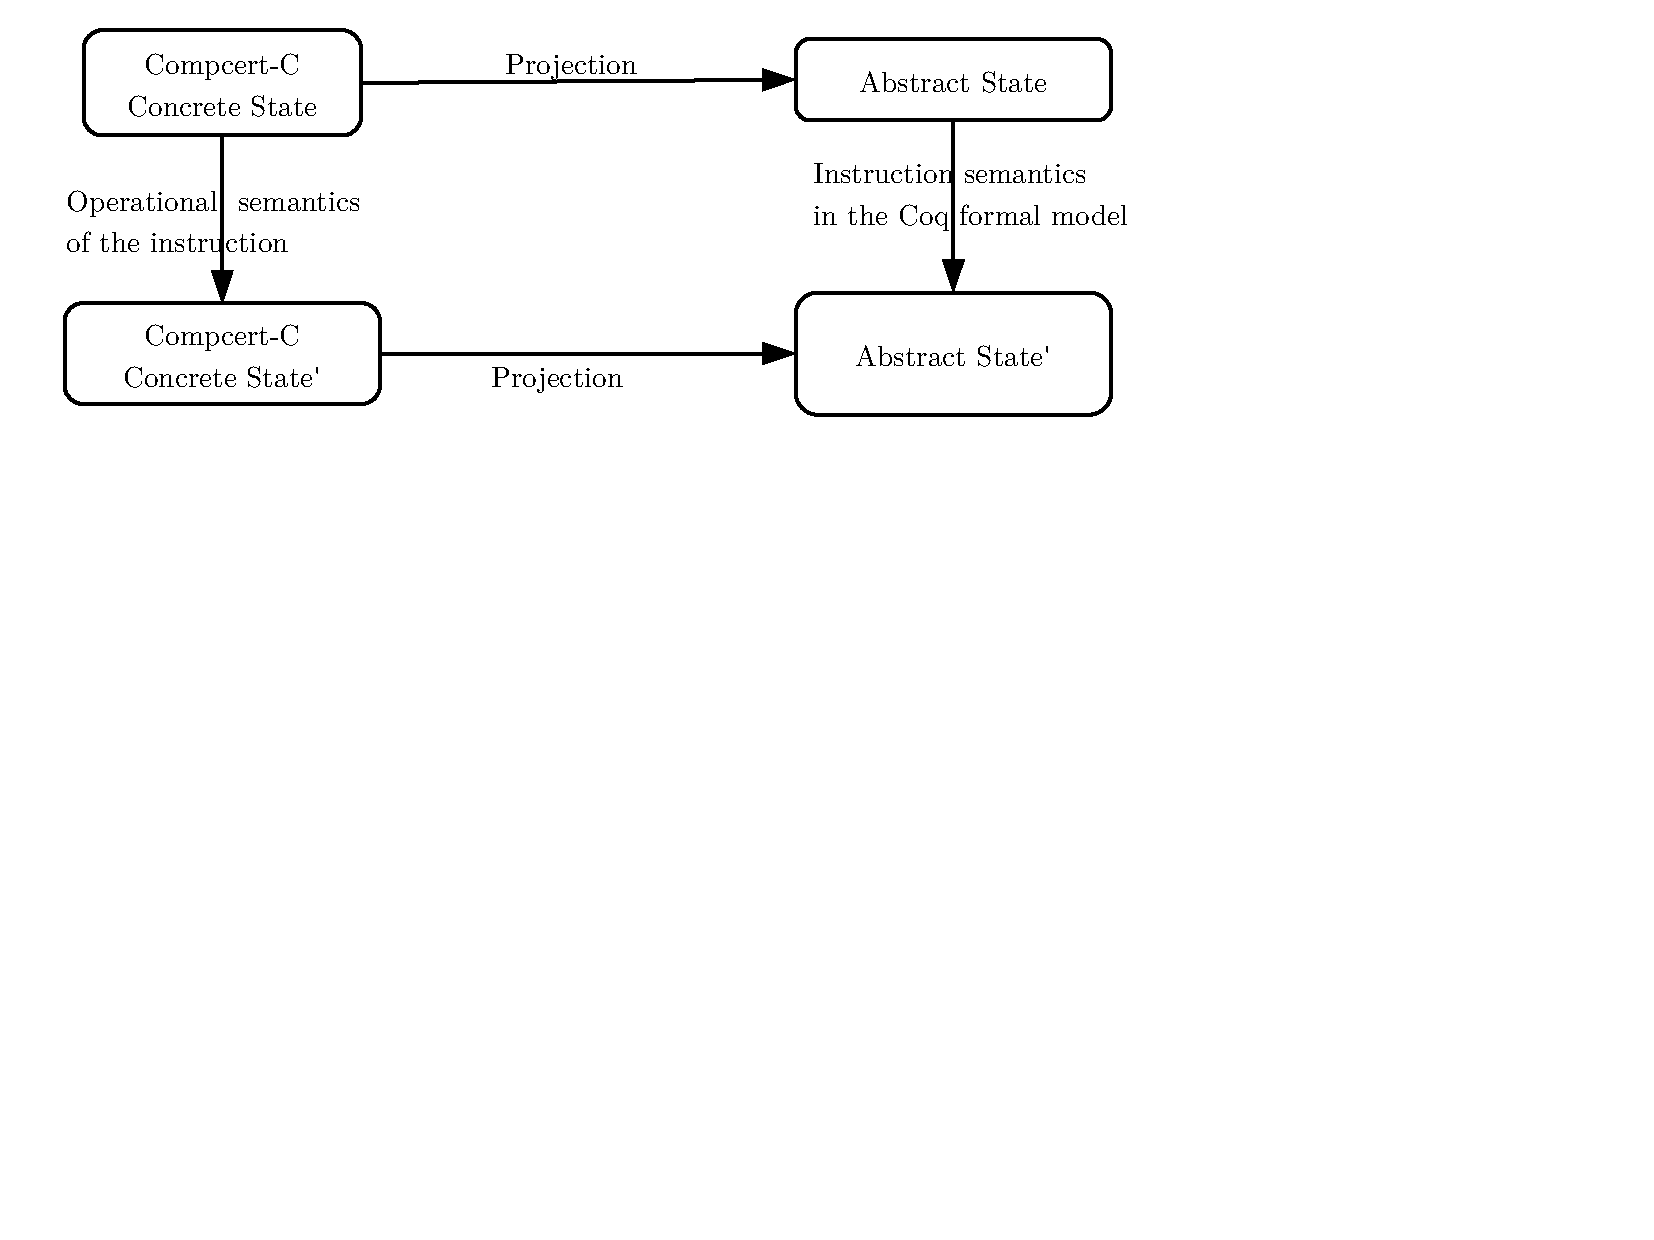
\includegraphics[width=0.9\linewidth, trim= 10mm 138mm 60mm 5mm, clip=true]{fig/newproj.pdf}
\caption{Theorem statement for a given ARM instruction}
\label{fig:theoca}
\end{figure}

The proof shall demonstrate that the operational semantics of the C
code corresponds to the ARM formal specification. The complete proof is
too lengthy for this article, and we only provide here an outline of
the method.  The state of the ARM V6 processor defined in the formal
model is called the \emph{abstract state}.  Alternatively, the same
state is represented by the data structures corresponding to C
semantics that we shall call the \emph{concrete state}.  In order to
establish correctness theorems we need to relate these two models.
Executing the same instruction on the two sides produces a pair of new
processor states which should be related by the same
correspondence. Informally, executing the same instruction on a pair
of equivalent states should produce a new pair of equivalent states,
as schematized by Figure~\ref{fig:theoca}.
%
Equivalent states are defined according to a suitable projection
from the C concrete state to the abstract model, as represented in
Figure~\ref{fig:proj}.
\begin{figure}[h]
\hfil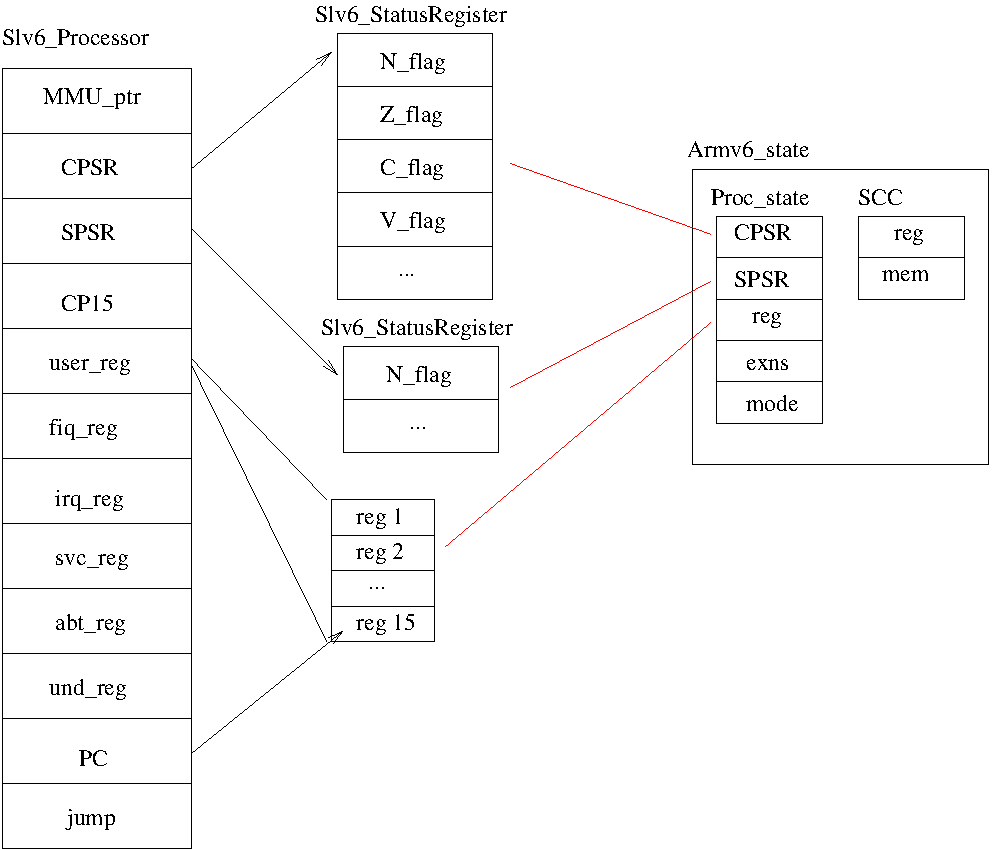
\includegraphics[width=.75\linewidth]{fig/projection.pdf}
\caption{Projection}
\label{fig:proj}
\end{figure}

\subsubsection{Projection}
In order to achieve a high speed simulation, the C ISS includes
optimizations. In particular, processor state representation in the C
implementation is complex, not only due to the inherent complexity of
the C language memory model, but also because of optimization and
design decisions targeting efficiency.  Despite the complexity of the
C memory model, the \compcert C semantics makes it possible to define
and prove the projection function. Fortunately, all of the
instructions operate on the processor state and there is a single
representation of that state in the simulator. It is necessary and
sufficient to prove the projection for each particular case of the
representation structure. For example, the projection of a register
performs a case analysis on possible values, whereas the projection of
saved data upon exceptions depends on the type of exception modes.
Although there are a number of specific cases to handle, the proof of
the projection is relatively straightforward.  In more detail:
\begin{itemize}
\item The C implementation uses large embedded \emph{struct}s to
  express the ARM processor state.  Consequently the model of the
  state is a complex Coq record type, including not only data fields
  but also proofs to verify access permission, next block pointer,
  etc.
\item Transitions are defined with a relational style (as opposed to a
  functional style where reasoning steps can be replaced by
  computations).
  % % JF: I feel the argument as somewhat dangerous, to be discussed.
  % % --> Xiaomu ?
  % As the kind of record type mentioned in the previous
  % item is too complex to execute computations with it, it is
  % convenient to describe the state transformations for memory with a
  % relation,
  % In simple situations functional style is lighter but its advantages
  % diminish in presence of dependent types.
  Relational style is more flexible,
  especially when dealing with constraints;
  and fits well with operational semantics.
\item The global state is based on a memory model with load
  and store functions that are used for read/write operations.
\end{itemize}

The proofs for instructions start from the abstract state described by
the formal specification.  To verify the projection of the
original state, we need the following data: the initial
memory state, the local environment, and the formal initial processor
state.  The projection is meaningful only after the C memory state is
prepared for evaluating the current function body representing a ARM
instruction.  In the abstract Coq model, we directly use the processor
state \texttt{st}.  But on the C side, the memory state is described
by the contents of several parameters, including the memory representation
of the processor state.  We also need to observe the modifications of
certain memory blocks corresponding to local variables.

% Fortunately \compcert formalizes the C memory model.
The semantics of \compcert C considers two environments. The global
environment \emph{genv} maps global function identifiers, global
variables identifiers to their blocks in memory, and function pointers
to a function definition body.  The local environment \emph{env} maps
local variables of a function to their memory blocks reference.  It
maps each variable identifier to its location and its type, and its
value is stored in the associated memory block.  The value associated
to a C variable or a parameter of a C function is obtained by applying
\texttt{load} to the suitable reference block in memory.  These two
operations are performed when a function is called, building a local
environment and an initialized memory state. When the program starts
its execution, \emph{genv} is built.  The local environment \emph{env}
is built when the associated function starts to allocate its
variables. Therefore, on the concrete side, a memory state and a local
environment is prepared initially using two steps. First, from an
empty local environment, all function parameters and local variables
are allocated, resulting into some memory state and the local
environment. Second, function parameters are set up using a dedicated
function \texttt{bind\_parameters} and the initial state is thus
created.

\subsubsection{Lemmas Library}
Next, we need to consider the execution of the instruction.
In the C ISS, there is a standalone C function
for each ARM V6 instruction.  Each function (instruction) has its own
correctness proof.  Each function is composed of its return
type, arguments variables, local variables, and the function body. The
function body is a sequence of statements including assignments and
expressions. Let us consider as an example the ARM instruction
\texttt{BL} (\texttt{Branch and Link}). The C code is:
%% JF HERE WE HAD A WRONG \small{ ==> scope until the end !!
{\small
\begin{verbatim}
void B(struct SLv6_Processor *proc,
       const bool L,
       const SLv6_Condition cond,
       const uint32_t signed_immed_24){
 if (ConditionPassed(&proc->cpsr, cond)){
  if ((L == 1))
   set_reg(proc,14,address_of_next_instruction(proc));
   set_pc_raw(proc,reg(proc,15)+(SignExtend_30(signed_immed_24)<<2));
 }
}
\end{verbatim}
}

\compcert has designed semantics for \compcert C in big-step inductive
types for evaluating expressions, which we reuse for the proof.  The
semantics is defined as a relation between an initial expression and
an output expression after evaluation.  Then, the body of the function
is executed.  On the concrete side, the execution yields a new state
\textbf{mfin}.  On the abstract side, the new state is
obtained by running the formal model.
% The formal model of ARM V6 is defined as a much simpler functional
% model and computing the value of a component can be performed
% directly.
We have to verify that the projection from the
concrete state \textbf{mfin} is related to this abstract
state.
% Note that all projections are
The proof is performed in a top-down manner. It follows the definition
of the instruction, analyzing the expression step by step.  The
function body is split into statements and then into expressions.
When evaluating an expression, one has to search for two kinds of
information. The first one is how the memory state changes on the
concrete side; the other is whether the results on the abstract and
the concrete model are related by the projection.  To this end, a
library of lemmas had to be developed, identifying five categories
summarized below.

%\begin{enumerate}
%\item
\medskip\noindent
  \textit{1. Evaluating a \compcert expression with no modification on the memory state.}\\
  Such lemmas are concerned with the expression evaluation on \compcert
  C side and in particular the C memory state change issue.  Asserting
  that a memory state is not modified has two aspects: one is that the
  memory contents are not modified; the other is that the memory
  access permission is not changed.  For example, evaluating the
  boolean expression $Sbit~==~1$ returns an unchanged memory state.
\[
\begin{array}{l}
\textrm{if}~~ G,E~\vdash \texttt{eval\_binop}_c~(Sbit~==~1),
\:M~\xLongrightarrow{\varepsilon}~v,\:M'
\\
\textrm{then}~~ M=M'.
\end{array}
\]
In Coq syntax, the relation in premise is expressed with
\texttt{eval\_binop}.
%a companion predicate of \texttt{exec\_stmt} above, devoted to binary operations.
In this lemma and the following,
$E$ is the local environment, $G$ is the global environment, $M$ is
the memory state, $\varepsilon$ is the empty event
% (\texttt{Events.E0} in Coq syntax);
(we may have here a series of events, e.g. system call, volatile
load/store) and $v$ is the result.
%(we may have here a series of events) and $v$ is the result.
% Here, $vres$ is not important.
The evaluation is performed under environments $G$ and $E$.  Before
evaluation, we are in memory state $M$.  With no event occurring, we
get the next memory state $M'$. According to the definition of
\texttt{eval\_binop}, an internal memory state will be introduced.
\begin{center}
$\dfrac
{G,E~\vdash a_1,M\Rightarrow M'~~~G,E~\vdash a_2,M'\Rightarrow M''
}
{G,E~\vdash (a_1~binop~a_2),M\Rightarrow~M''}$
\end{center}

In the example, expression $a_1$ is the value of $Sbit$ and $a_2$
is the constant value $1$.  By inverting the hypothesis of type
\texttt{eval\_binop}, we obtain several new hypotheses, including on
the evaluation of the two subexpressions and the introduction of an
intermediate memory state $M''$.  Evaluating them has no change on the
C memory state, hence we have $M = M'' = M'$.
In more detail, from the \compcert C semantics definition, we know that
the evaluation of an expression will change the memory state
if the evaluation contains uses of \texttt{store\_value\_of\_type}.
% in \compcert versions before 1.11.
% which stores the value in memory at a given block reference and
% memory chunk.
In \compcert, the basic store function on memory
is represented by an inductive type \texttt{assign\_loc} instead of
\texttt{store\_value\_of\_type}.
As a note, since \compcert version supports volatile memory access,
we also have to determine whether the object type is volatile before storage.
% and also type size in addition of the access mode.

%\item
\medskip\noindent
\textit{2. Result of the evaluation of an expression with no modification on the memory.}\\
Continuing the example above, we now discuss the result of evaluating
the binary operation $Sbit~==~1$ both in the abstract and the concrete model.
At the end of evaluation, a boolean value $true$ or $false$ is returned
in both the concrete and the abstract models.
\[
\begin{array}{l}
\textrm{if} ~ \texttt{Sbit\_related}~M~\texttt{Sbit},\\
\textrm{and} ~ G,E~\vdash \texttt{eval\_rvalue\_binop}_c~(Sbit~==~1),  M\Rightarrow~v,M'\\
\textrm{then} ~ v=(Sbit~==~1)_{coq}
\end{array}
\]
Intuitively, the projection corresponding to the parameter
\texttt{sbit} in the concrete model must yield the same value as in
the abstract model.  Here, the expression is a so-called ``simple
expression'' that always terminates in a deterministic way, and
preserves the memory state.  To evaluate the value of simple
expressions, \compcert provides two big-step relations
\texttt{eval\_simple\_rvalue} and \texttt{eval\_simple\_lvalue} for
evaluating respectively their left and right values.  The rules have
the following shape:
\[
\dfrac{
\begin{array}{l}
G,E~\vdash a_1,M\Rightarrow v_1 \quad G,E~\vdash a_2,M\Rightarrow v_2\\
\texttt{sem\_binary\_operation}(op,v_1,v_2,M)~=~v
\end{array}}
{G,E~\vdash (a_1~op~a_2),M\Rightarrow v}
\]
In order to evaluate the binary expression $a_1~op~a_2$,
the sub-expressions $a_1$ and $a_2$ are first evaluated,
and their respective results $v_1$ and $v_2$ are used
to compute the final result $v$.

%\item
\medskip\noindent
  \textit{3. Memory state changed by storage operation or side effects.}\\ % of evaluating expression
  As mentioned before, evaluating some expressions such as
  \texttt{eval\_assign} may modify the memory state.  Lemmas are
  required to state that corresponding variables in the abstract and
  in the concrete model must evolve consistently.  For example,
  considering an assignment on register $Rn$, the projection relation
  \texttt{register\_related} is used. Expressions with side effects of
  modifying memory are very similar.
\[
\begin{array}{l}
\textrm{if} ~~ \texttt{rn\_related}~M~rn\\
\textrm{and}~~  G,E~\vdash \texttt{eval\_assign}_c~(rn:=rx),M~\Rightarrow~ M',v\\
\textrm{then} ~~ \texttt{rn\_related}~M'~rn
\end{array}
\]

%\item
\medskip\noindent
  \textit{4. Internal function call.}\\
  The simulation code is sometimes using functions from libraries.
%  One needs to verify potential issues from these calls.
  We   distinguish \texttt{internal} functions and \texttt{external}
  functions.  An internal function is a function that belongs to a
  library, the code of which is part of the simulator, that we have
  coded ourselves, or the C code is provided by compcert C.  An
  external function is a function for which we do not have access to
  the operational semantics.  After an internal function is called, a
  new stack of blocks is typically allocated in memory.  After the
  evaluation of the function, these blocks will be freed.
  Unfortunately, this may not bring the memory back to the previous
  state: the memory contents may stay the same, but pointers and
  memory organization may have changed.
  \label{page:libfunast}
  \[
  \begin{array}{l}
    \textrm{if} ~~  \texttt{proc\_state\_related}~M~st \\
    \textrm{and} ~~ G,E~\vdash \texttt{eval\_funcall}_c (copy\_StatusRegister)_c,M\Rightarrow~v,~M'\\
    \textrm{and} ~~ st'~=~(copy\_StatusRegister)_{coq}~st\\
    \textrm{then} ~~\texttt{proc\_state\_related}~M'~st'.
  \end{array}
  \]

  Lemmas must be developed regarding the evaluation of internal
  functions, so that one can observe the returned results,
  compare it with the corresponding evaluation in the formal
  specification, and verify some conditions.  For example, the lemma
  above is about the processor state after evaluating an internal
  function call \texttt{copy\_StatusRegister}, which reads the value of
  the CPSR (Current Processor Status Register) and copies it into
  the SPSR (Saved Processor Status Register) when an exception occurs.  The
  evaluation of \texttt{copy\_StatusRegister} must be protected by a
  check on the current processor mode.  If it is in authorized mode, the
  function \texttt{copy\_StatusRegister} can be called.  Otherwise, the
  result is ``unpredictable'', which is defined by ARM architecture

  It is necessary to reason on the newly returned states, which
  should still be related by the projection.  This step is usually easy
  to prove, by calculation on the two representations of the processor
  state to verify that they match.

%\item
\medskip\noindent
  \textit{5. External function call.}\\
  The \compcert C AST of an external function call contains the types
  of input arguments and of the returned value, and an empty body.
  For each external function (e.g. \texttt{memcpy()}), we have its
  asserted properties. mostly provided by \compcert C.  The general
  expected properties of an external call are that (i) the call
  returns a result, which has to be related to the abstract state,
  (ii) the arguments must comply with the signature.  (iii) after the
  call, no memory blocks are invalidated, (iv) the call does not
  increase the access permission of any valid block, and finally that
  the memory state can be modified only when the access permission of
  the call is granted. For each external call, such required
  properties are verified.
%\end{enumerate}

%% JF Not crucial
% In addition to the above lemmas we had to prove a fair number of more
% trivial lemmas that are omitted here.  Most of them are related to the
% semantics of \compcert C. They are all gathered into a library of
% lemmas used to construct the individual instructions proofs.

\subsubsection{Inversion}
% Details are given in~\cite{xiaomu-phd}.
Equipped with these lemmas we can build the proof scripts for ARM
instructions.  For that, we are decomposing the ARM instruction
execution step by step to perform the execution of the C programs.
\compcert C operational semantics define large and complex inductive
relations. Each constructor describes the memory state transformation
of an expression, statement, or function.  As soon as we want to
discover the relation between memory states before and after
evaluating the C code, we have to \emph{invert} the hypotheses of operational
semantics to follow the clue given by its definition, to verify the
hypotheses relating concrete memory states according to the
operational semantics.

% During the development of a proof, if a hypothesis is an instance of
% an inductive predicate and we want to derive the consequences of this
% hypothesis, the general logical principle to be used is called
% \emph{inversion}.
An \emph{inversion} is a kind of forward reasoning
step that allows for users to extract all useful information contained
in a hypothesis.  It is an analysis over the given hypothesis according
to its specific arguments, that removes absurd cases, introduces
relevant premises in the environment and performs suitable
substitutions in the whole goal.
% The practical need for automating
%inversion has been identified many years ago and
Most proof assistants provide an inversion mechanism.
In the case of Coq, it is
a general tactic called
\inversion~\cite{coqmanual}.

Every instruction contains complex expressions, but each use of
\inversion will go one step only.  If we want to find the relation
between the memory states affected by these expressions, we have to
invert many times. For illustration, let us consider the simple
example from the ARM reference manual \texttt{CPSR = SPSR}, that
assigns to register CPSR the value of SPSR (defined above).  As the
status register is not implemented by a single value, but a set of
individual fields, the corresponding C code is a call to the function
\texttt{copy\_StatusRegister}, which sets the CPSR field by field with
the values from SPSR.  Lemma \texttt{same\_cp\_SR} below states that
the C memory state of the simulator and the corresponding formal
representation of ARM processor state evolve consistently during this
assignment.
\begin{alltt}\small
Lemma same_copy_SR :
  \(\forall\) e m l b s t m' v em,
  proc_state_related m e (Ok tt (mk_semstate l b s)) \(\rightarrow\)
    eval_expression (Genv.globalenv prog_adc) e m expr_cp_SR t m' v  \(\rightarrow\)
    \(\forall\) l b, proc_state_related m' e
                      (Ok tt (mk_semstate l b (Arm6_State.set_cpsr s
                                              (Arm6_State.spsr s em))))
\end{alltt}
In its proof, 18 consecutive inversions are needed in order to exhaust
all constructors occuring in the assumptions.  Unfortunately,
\inversion generates uncontrolable names which pollute proof scripts.
Here, an intensive use of \inversion makes proofs scripts
unmanageable, and not robust to version changes of Coq or \compcert.
%
In order to reduce the script size and get better
maintainability, we studied a general solution to the inversion problem,
and developed a new mechanism described in~\cite{itp13}.
%\cite{small-inversion,itp13}
% The standard inversion mechanism from Coq has been expanded into a new
% inversion tactic for inductive types in \compcert.  The semantics of
% \compcert C tells how the memory state is transformed by evaluating
% expressions.  Using the built-in constructs of the tactics language,
% one can define a high-level tactic for each inductive type, gathering
% all the functions defined for its constructors.
%
On top of it, we could program a Coq tactic able to
% The new tactic
automatically find the hypothesis to invert by matching the targeted
memory states,
properly manage other hypotheses,
perform our inversion,
clean up the goal,
and repeat
% then to revert related hypotheses,
% Next, all other related hypotheses are updated according to the new names,
% and finally new values and useless variables or hypotheses are cleaned up.
the above steps until all transitions between the
two targeted memory states are discovered.

As a result, proofs script have become much shorter and more manageable.
Considering the former example of \texttt{same\_copy\_SR},
the 18 calls to standard \inversion
reduce into one single step:
\texttt{inv\_eval\_expr~m~m'}.
\subsubsection{Instruction Proofs}
Proofs of instructions rely heavily on
the library of lemmas and the controlable inversion mechanism
described above.
Scripts size vary with the instructions complexity from less than 200 lines (e.g
170 for LDRB) to over 1000 (1204 for ADC).
As a result, for each ARM instruction,
we have established a theorem proving that the C code
simulating an ARM instruction is equivalent to the formal
specification of the ARM processor.


%%%%%%%%%%%%%%%%%%%%%%%%%%%%%%%%%%%%%%%%%%%%%%%%%%%%%%%%%%%%%%%%%
\section{Conclusion}
\label{conclusion}

The SimSoC virtual prototyping software is a full system simulation
framework. Based on SystemC and TLM, it contains fast instruction set
simulators and a library of models for other hardware components such
as RS232 controller, or network controllers. Thanks to TLM interfaces,
these models can interact with other third party models to elaborate
complete simulation platforms that can run an operating system
starting from a bootloader.

\simsoc can fully simulate a complete hardware platform. In addition
to the ISS, it also includes implementation of several Memory
Management Units (MMU's), interrupt controllers, serial line and
network controllers.  All of these simulation models are implemented
as SystemC modules using transaction modeling. As a proof of concept,
we have developed several simulators to simulate commercially
available System-on-Chips. All of the SoC's models developed are
running the Linux operating system, using the Linux binary as is for
the commercial chip. In order to boot Linux, it is also possible to
use a boot loader such as U-Boot.  The SoCs available are:
\begin{itemize}
\item the SPEArPlus 600 circuit from ST Microelectronics.  This SoC
  contains among other components two ARM926 subsystems (dual core),
  together with various peripheral controllers.
\item the Texas Instrument AM1705 circuit. For this SoC, we have also
  developed an Ethernet controller model, and a bridge to real
  Internet so that we can test the simulated platform connected to
  real machines on the network, thanks to a bridge with the local
  Ethernet port.
\item the FreeScale 8641D dual core Power architecture chip.
\item We have under construction an example of the Power ez200 series,
for which we develop an Approximately Timed version.
\end{itemize}
In order to build faithful virtual prototypes, we have added to SimSoc
a proven generated simulator of the ARM instruction set.

Using the approach presented here, we can construct a tool chain that
makes it possible to certify that the simulation of a binary
executable program on some simulation platform is compliant with the
formal model of the target hardware architecture.  Using Compcert-C,
that has defined formal C semantics, we have formally proved, using
the Coq theorem prover to automate the proof, the ARM v6 Instruction
Set Simulator of SimSoc.

Given that we have a proof that the machine code generated from C is
correct, thanks to \compcert, and now a proof of the ARM instruction
set for these instructions, we have a proof that the simulation of an
algorithm on our simulator is conforming to the algorithm for the
target architecture.  With this technique, there is no limit on the
size of the C code that can be verified.  In fact, if there existed a
publicly available formal model of the ARM processor approved by ARM
Ltd company, our work, combined with CompCert C compiler, could be
construed to define a {\em verified execution of a C program}, that
could be used for certification procedures.

We certainly acknowledge the limits of our approach: the quality of
our ``verified simulation'' relies on the faithfulness of our formal
model of the ARM processor to the real hardware. Because the vendor
companies do not provide a formal description of their hardware, one
has to build them\footnote{Note that this problem is the same as for
  the work done by Cambridge University.}.  This issue is partly
solved in this work by automatically deriving the most tedious parts
of the Coq formal model from pseudo-code extracted from the vendor
reference manual.  If the vendors would make public formal
specifications of their architectures, then our toolchain would become
fully verified.

We believe this work has further impact on proofs of programs.  First,
we have proved here a significantly large C program.  Second, because
the proved program is a hardware simulator, it can be used as a tool
to prove execution of target programs.  For example considering a
cryptographic algorithm implemented for the ARM archiecture and
compiled with Compcert-C, it could then be proved that the execution
of that program provides the exact encryption required, and nothing
else.  Therefore, the tool presented is an enabler for the proofs of
other programs, which offers a direction for future research.

Another consequence of this work is that, supposing one could
compile the C instructions to silicon using a silicon compiler,
and that compiler would also be certified, ala \compcert,
it would then make it possible to prove real hardware...


\subsection{Acknowledgements}
This work has been partly funded by the international collaboration support
of France ANR and NSFC China in the SIVES project.

\bibliographystyle{splncs03}
\bibliography{references}

% \bibliographystyle{IEEEtran}
% \bibliographystyle{abbrv}
% \bibliography{references}

\end{document}
